\section{When does a parameter become a measurement?}
\label{sec:measurement}

\begin{figure}[!htb]
\centering
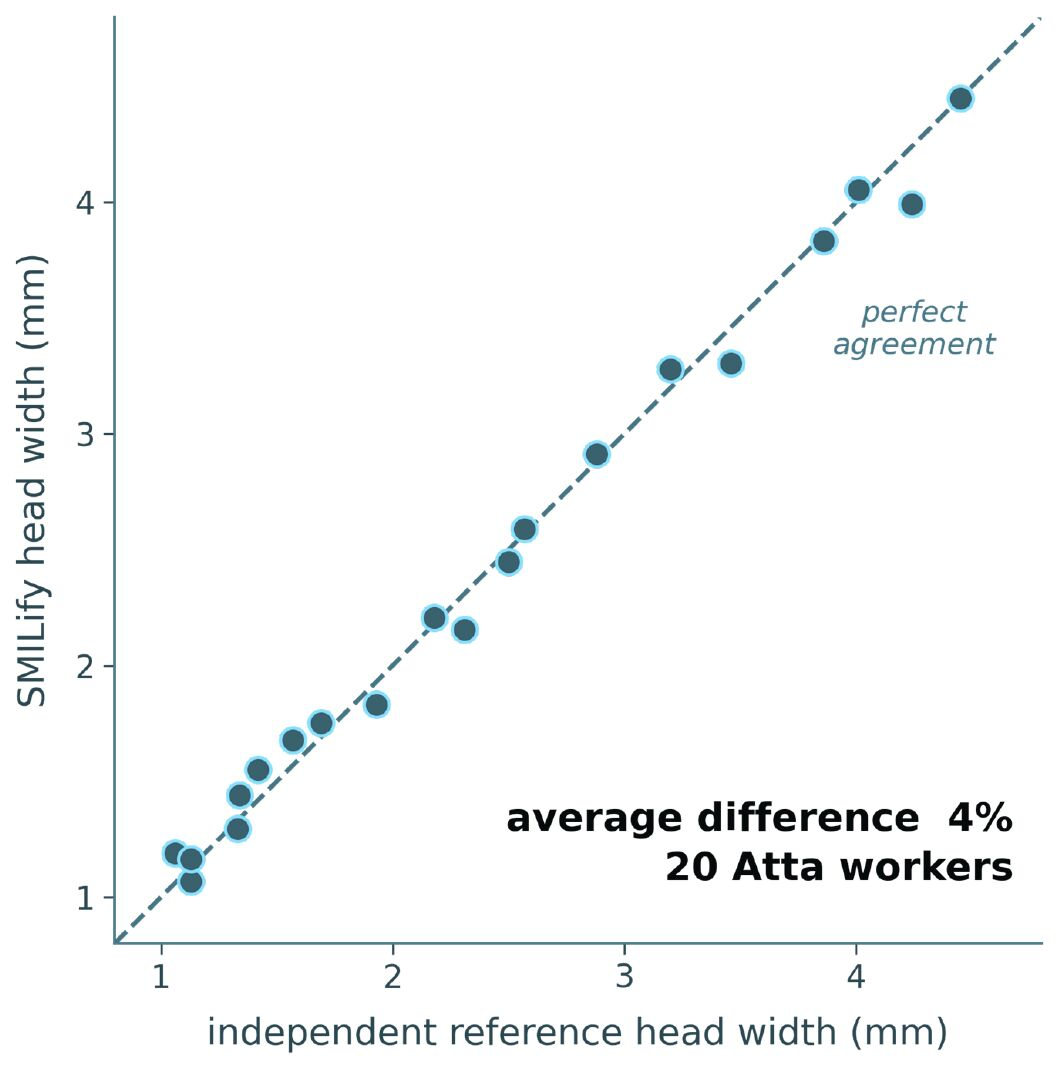
\includegraphics[width=0.6\linewidth]{figures/fig_parameter_measurement.jpg}
\caption{Head width read directly from 20 fitted \emph{Atta} workers against
an independent physical reference measurement.}
\label{fig:parameter-measurement}
\end{figure}

A fitted parametric model is not an end in itself; it is an instrument.
Once every specimen occupies the shared coordinate system of
\S\ref{sec:pipeline-overview}, quantities entomologists currently extract
manually under a microscope (head width, body length, appendage
proportions) become extractable automatically and at population scale,
\emph{provided} the extracted numbers agree with what a caliper would
report. This is the check that closes the chain this report has followed
throughout: \textbf{registration} $\rightarrow$ \textbf{measurement}
$\rightarrow$ \textbf{biological value}.

On a 20-specimen \emph{Atta} worker corpus, joint positions recovered
directly from the fitted model reach a median error of $1.05\%$ of Weber's
length against expert reference measurements, with $96\%$ of joints within
$5\%$, consistent with the coxa-and-body-axis end of the regional error
profile in Table~\ref{tab:regional-error}, on a corpus with less of the
distal-appendage difficulty that dominates the harder end of that table.
Two independent allometric relationships (head width against body
length, and head width against body mass) reproduce published reference
slopes closely ($1.189$ vs.\ $1.235$, and $0.380$ vs.\ $0.395$
respectively), with $R^2$ between $0.987$ and $0.993$. Figure~\ref{fig:parameter-measurement}
shows the same agreement directly, in absolute units: a mean difference of
$4\%$ between SMILify-derived and independently measured head width.

Two further checks were made before treating this agreement as settled. The
first compared two competing definitions of ``head width'': one read from
the model's own joint-derived reference points, the other from an
alternative purely geometric definition. The joint-derived definition showed
a smaller bias against the physical reference ($-0.13\%$) than the
geometric one ($+2.22\%$), so it is the definition used throughout this
report. The second check is a methodological one worth stating generally:
raw agreement in millimetres can partly be inherited from shared
whole-body-length scaling rather than from an independently accurate
measurement, so a \emph{dimensionless} ratio such as head width over body
length is a more informative validation target than absolute agreement
alone, and is reported alongside it here for that reason.
